\section{Evaluation}
\label{sec:eval}

\subsection{Experimental Setup}
\textbf{Evaluation Methodology.}
In this part, we first systematically evaluate the effectiveness of out system, then provide a detailed analysis to evaluate its robustness against attackers with different capabilities. We also test our system under various variables. At last, a case study is conducted in a common office to validate the our system's practicality.

Please note that the inconsistency in the accuracy of Tencent ASR across experiments is caused by differences in test sets and test dates. But for each experiment, the test set is consistent and is done within a short time period.

\textbf{Dataset.}
We adopt 6 widely-used datasets in different parts of this section. LibriSpeech~\cite{LibriSpeech} is used in the baseline and other unmentioned parts. AISHELL-1~\cite{aishell_2017} (Mandarin), Multilingual LibriSpeech~\cite{mls2020_interspeech} (Portuguese), and Japanese Versatile Speech~\cite{takamichi2019jvs} are used for testing different languages.
TIMIT~\cite{timit} is used in Section~\ref{subsec:robustness_adversarial_training} because of its small size which can make machine learning models converge faster. Harvard Sentences~\cite{harvard_sentences} is used for human perception test because of its short sentences, which can reduce the difficulty for human to recognize.

\textbf{Dataset Preprocessing.}
Before generating noise, we need to first segment the corpus into phonemes. We segment the English corpus (LibriSpeech and Harvard Sentences) with Prosodylab Aligner~\cite{prosodylab_aligner} and Mandarin corpus with Charsiu~\cite{zhu2022charsiu}. For Portuguese and Japanese, we adopt the Montreal Forced Aligner~\cite{MFA}. The TIMIT dataset provides aligned phonemes initially. We separate the phonemes into vowels and consonants after segmentation according to the International Phonetic Alphabet (IPA).

\subsection{Effectiveness}
\label{subsec:baseline}

\textbf{Overall Performance.}
We first evaluate our noise in the single-user scenario. We test the jamming performance of our noise under different ASRs and use a [0, 8] kHz band-limited gaussian white noise for comparison. A test set containing 27000 words is generated from LibriSpeech.
Since built-in noise reduction mechanism of recording devices may affect the reception of white noise (proven in Fig~\ref{fig:white_denoise}), we directly mix noises with speech signal in digital domain and feed the mixed signals to ASRs for a fair comparison.

We test four commercial ASR systems (Amazon Transcribe \cite{aws}, Tencent ASR \cite{tencent_asr}, Xunfei ASR \cite{xunfei_asr} and Google Speech-to-Text \cite{google_stt}) and two commonly used open source ASR systems (DeepSpeech \cite{deepspeech} and WeNet \cite{yao2021wenet}). The results in Figure \ref{fig:digital_result_different_SNR} show that our noise performs significantly better than white noise when $SNR \leq 4$, and the gap between them gradually increases as the SNR decreases. Besides, the advantage of our noise is more obvious on commercial ASRs than on open-source ones. We suppose this is because commercial systems have been enhanced for the interference of white noise.

\begin{figure*}[t]
    \centering
    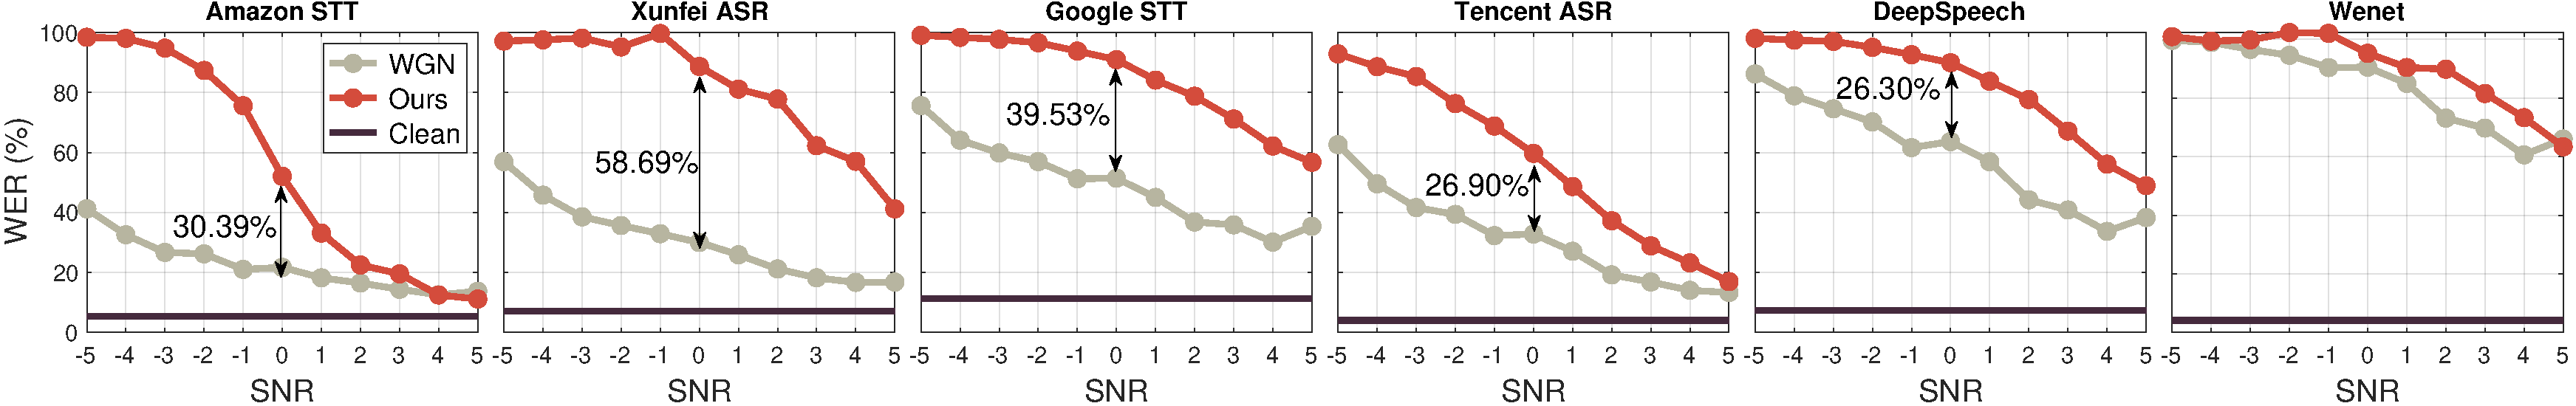
\includegraphics[width=1\linewidth]{images/digital_all_data.pdf}
    \caption{Recognition results of different ASR systems. We use the clear audio as a baseline.}
    \label{fig:digital_result_different_SNR}
    \vspace{-5mm}
\end{figure*}

\textbf{Different Languages.}
We choose other three languages from different language families to ensure sufficient phonemic diversity. In addition to English (West Germanic language in Indo-European language family), we test Mandarin (Sino-Tibetan language family), Portuguese (Western Romance language in Indo-European language family) and Japanese (Japonic language family). We randomly choose 200 audios from each dataset as the test set and mix them with corresponding noises under different SNRs. Specifically, we recognize the Portuguese data with Amazon Transcribe because of its good performance on clean Portuguese corpus. The result in Figure~\ref{fig:multi_language} shows that our jamming method performs well in different languages.
\begin{figure}[t]
    \centering
    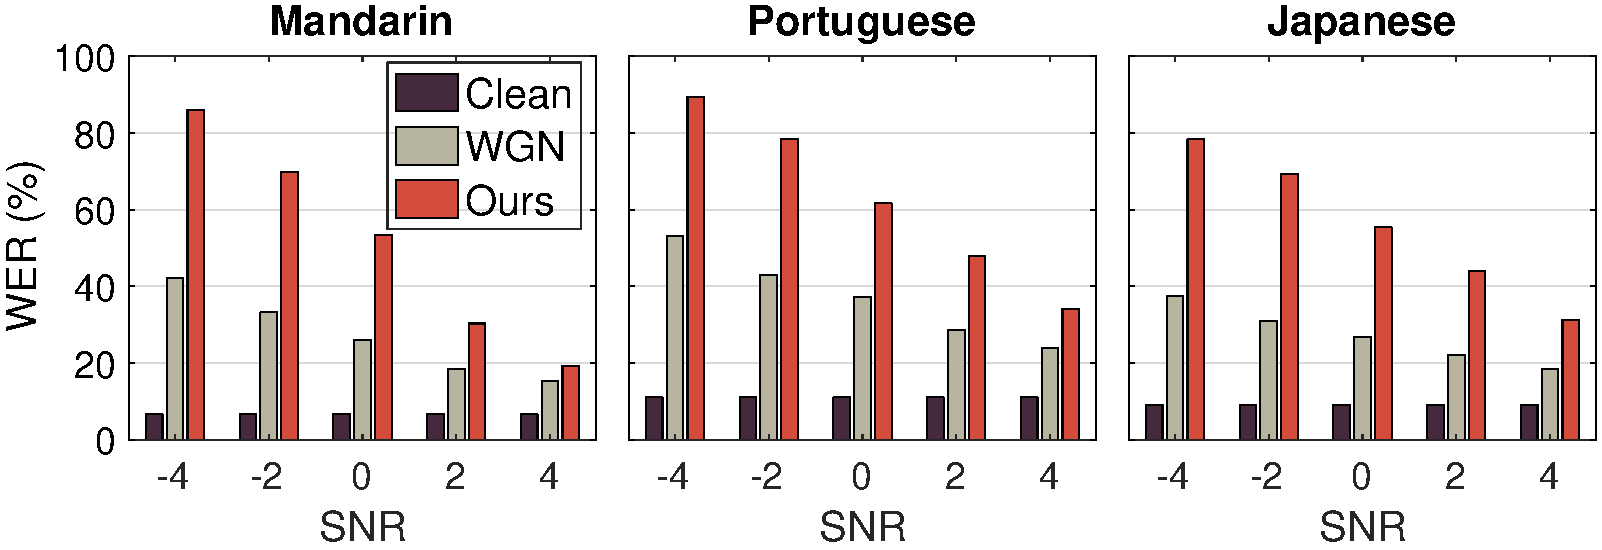
\includegraphics[width=\linewidth]{images/multi_language.pdf}
    \caption{Results when applying on different languages. White gaussian noise (WGN) is also tested for comparisons.}
    \label{fig:multi_language}
\end{figure}
    

\textbf{Multi-User Scenario.}
We evaluate our system with different number of randomly chosen users.
The results in Figure~\ref{fig:multi_user_result} shows that when the number of users is smaller than 10, the jamming effectiveness is lower than that of the single user scenario where the noise is generated based on the target person's speech, but significantly higher than the noise generated from the speech data of the other person with the same sex. When the number of users is greater than 10, the noise's jamming effectiveness gradually approaches to the noise generated from the people with the same sex.

\begin{figure}[t]
    \centering
    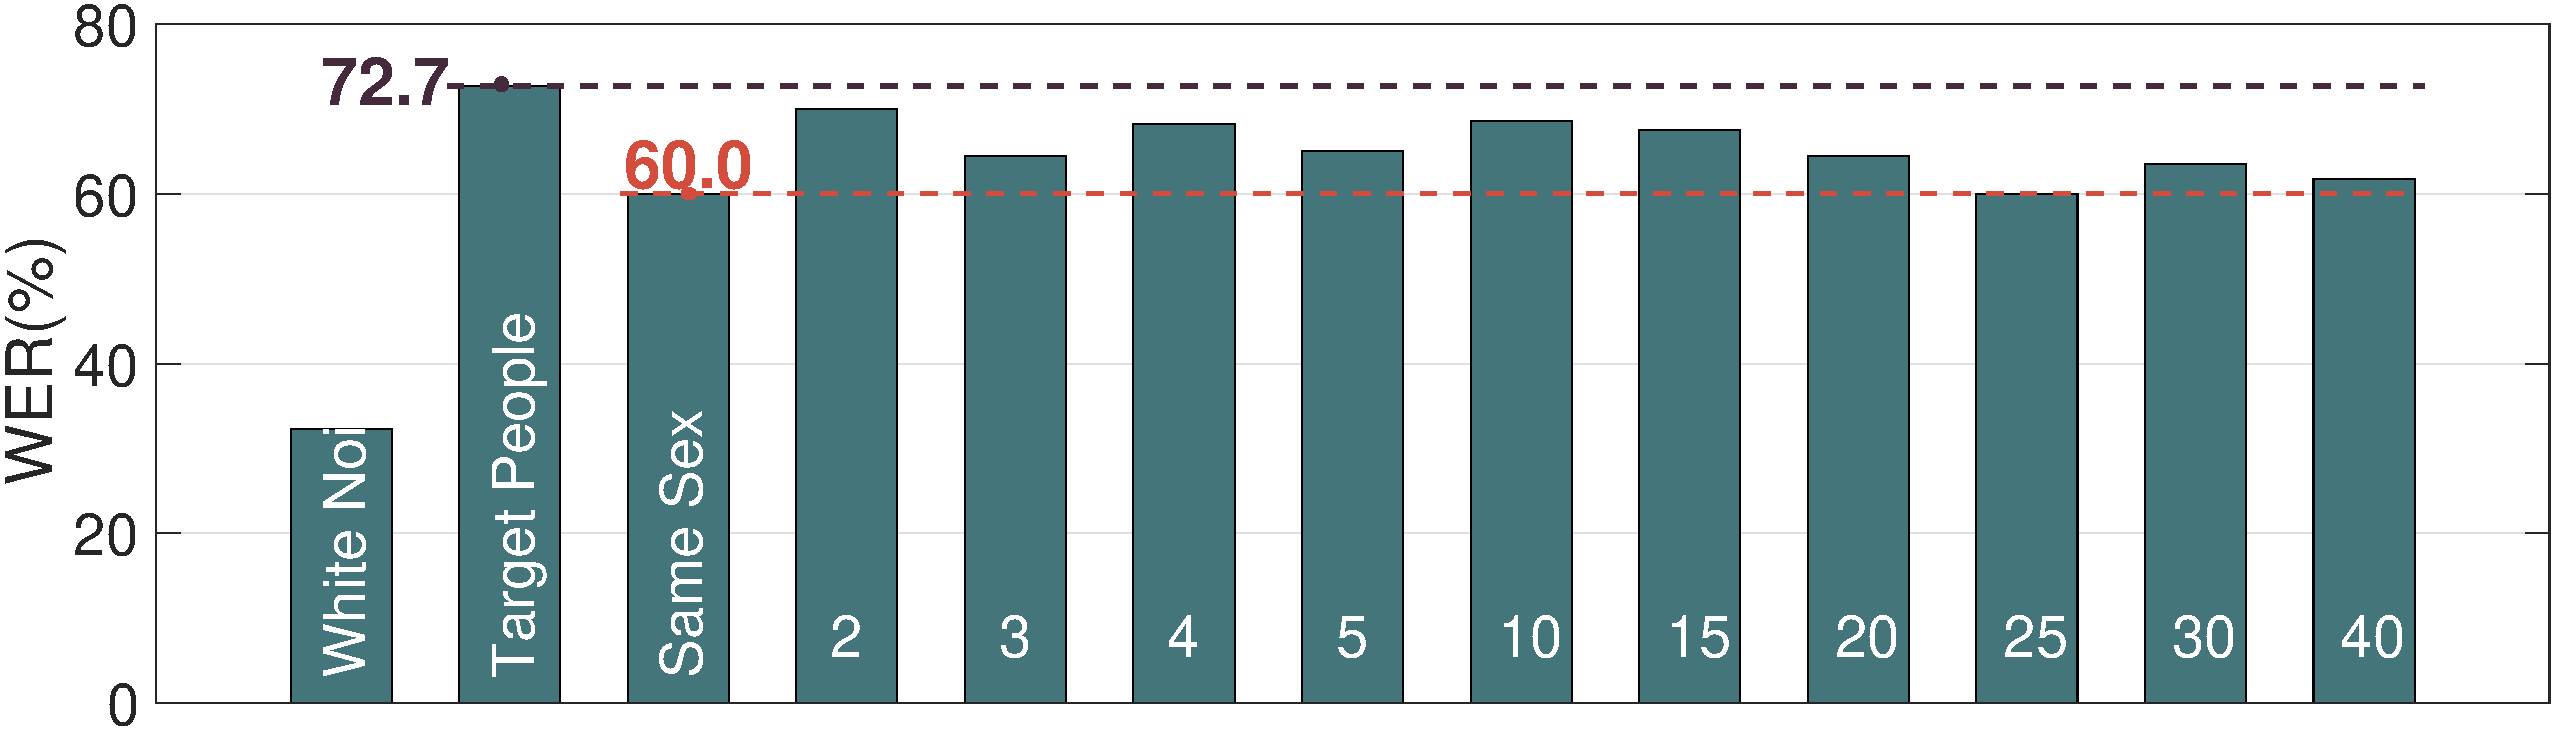
\includegraphics[width=\columnwidth]{images/multi_user_results.pdf}
    \caption{Recognition results for multi-user scenario. The numbers in the bar represent the number of user.}
    \label{fig:multi_user_result}
    \vspace{-5mm}
\end{figure}

\textbf{Real-World Scenario.} We place a smartphone around the transmitter array and adjust the transmitter's energy to get different SNRs. We use another smartphone to play speech signals. As it is hard to get a stable and precise SNR in real-world scenario, we test several times in each SNR interval and then calculate the average and the minimum WER. We collect more than 70 hours data in totally. The results in Table \ref{tab:real_world_wer} show that when $SNR < 0$, the WER in real-world scenario is slightly lower than that in the digital domain, but significantly higher when $SNR > 0$. 

\begin{table}[h]
    \vspace{-3mm}
    \caption{Recognition result in real-world scenario.}
    \centering
    \resizebox{\columnwidth}{!}{
        \begin{tabular}{cccccccc}
        \toprule
        \textbf{SNR}         & \textbf{\textless{}-4} & \textbf{{[}-4,-2{]}} &\textbf{ {[}-2, 0{]} }&\textbf{ {[}0,2{]}} &\textbf{{[}2,4{]}} & \textbf{\textgreater{}4 }&\textbf{ Clear} \\ 
        \midrule
        \textbf{Avg WER(\%)} & 85.8          & 81.6        & 77.6        & 70.2      & 56.4      & 42.3            & 11.5  \\ 
        \textbf{Min WER(\%)} & 68.6          & 77.0        & 62.4        & 62.2      & 45.3      & 30.3            & -     \\ \hline \hline
        \textbf{Digital WER(\%)} & 88.6          & 85.4       & 68.8        & 48.67      & 28.9      & 17.0           & 4.1     \\ 
        \bottomrule
        \end{tabular}
    }
    \label{tab:real_world_wer}
    \vspace{-3mm}
\end{table}

\textbf{End-to-End Scenario.}
\label{subsubsec:real_world_end_to_end}
We further evaluate our system in a real-world end-to-end scenario with two volunteers (one male and one female). Each of them reads one sentence (about 5 seconds) randomly selected from~\cite{harvard_sentences} for registration. We extract their voice embeddings and then match the corresponding closest people in LibriSpeech for noise generation. To simulate a realistic scenario, we place the transmitter array on an office table and then place 5 smartphones acting as eavesdroppers with different distances to the array. We have the volunteer sit at the table and read 50 sentences selected from~\cite{harvard_sentences}. As it is hard to control the SNR precisely in a real-world scenario, we record the noise and speech separately and then mix them under various SNRs. The recognition results of the mixed audios (i.e., jammed speech) are shown in Figure~\ref{fig:end_to_end}.  The results show that our system performs well in the real-world end-to-end scenario.

\begin{figure}[t]
    \centering
    \begin{subfigure}[t]{0.49\linewidth}
        \centering
        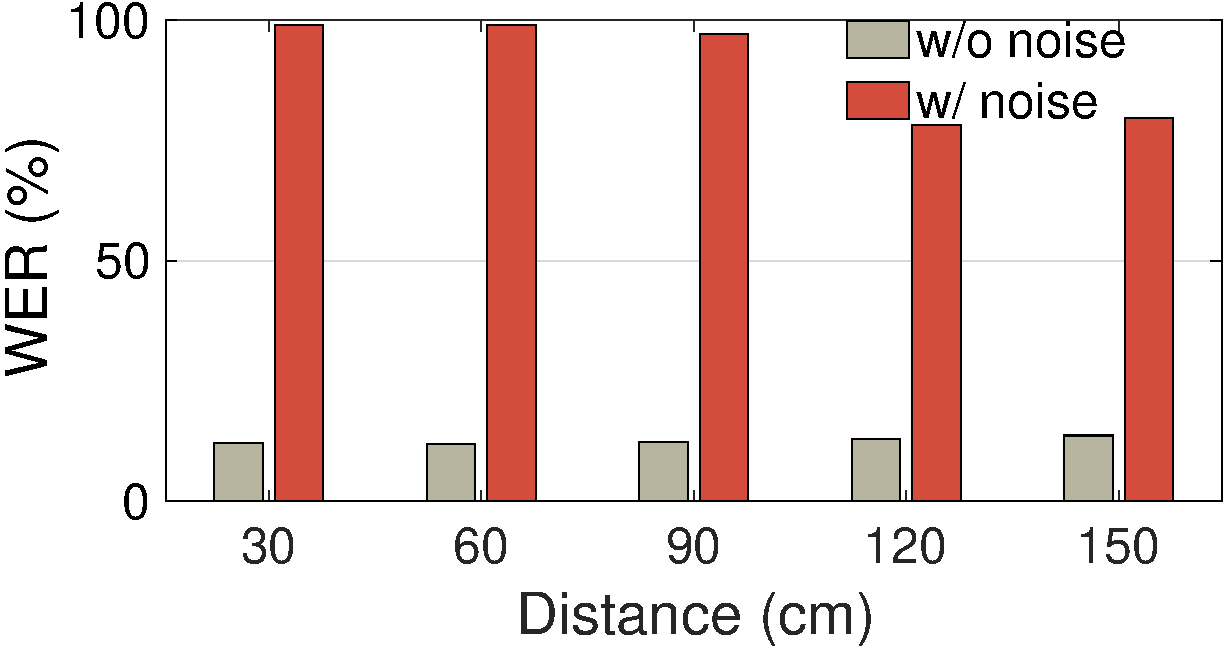
\includegraphics[width=\linewidth]{images/end_to_end.pdf}
    \end{subfigure}
    \begin{subfigure}[t]{0.49\linewidth}
        \centering
        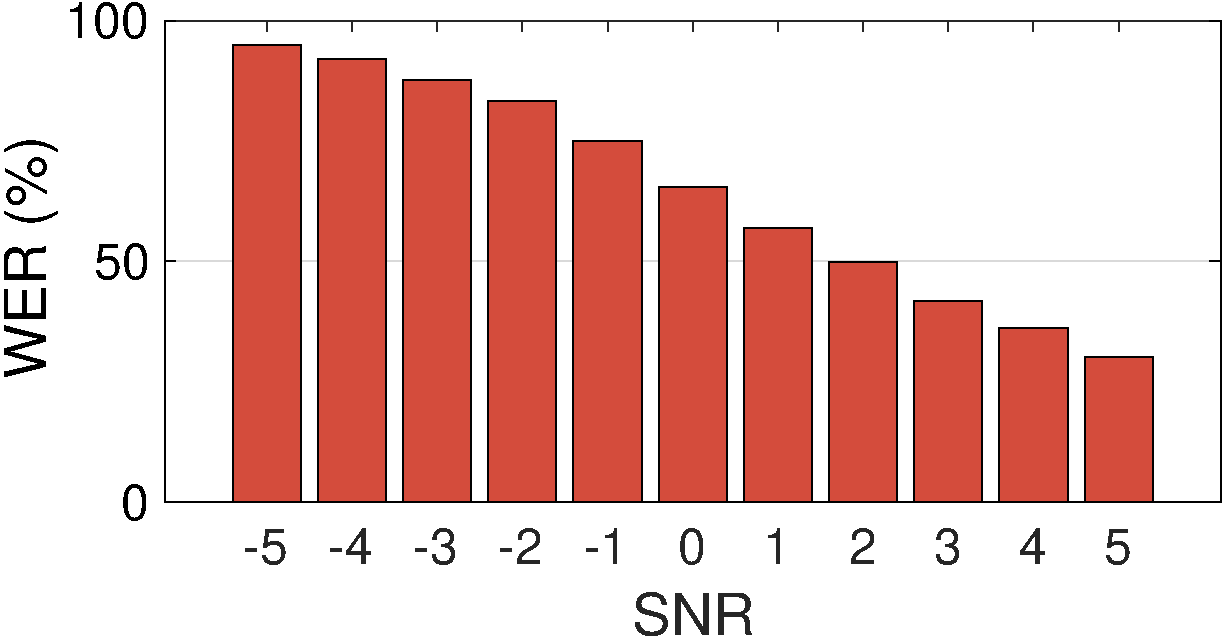
\includegraphics[width=\linewidth]{images/end_to_end_snr.pdf}
    \end{subfigure}
    \caption{Results of the end-to-end scenario. Left: results in different distances. Right: results in different SNR.}
    \label{fig:end_to_end}
    \vspace{-5mm}
\end{figure}

\textbf{Human Perception.} We recruit 15 testees including 5 females and 10 males aged from 22 to 31 to test the recognizability of jammed audios. To make testees put their effort into the study, we adopt an accuracy-related reward to incent them. Tested audios are either generated in digital domain or recorded over-the-air. In the digital domain, in addition to white noise and our noise generated with the target's speech, we also test our noise generated from audios of same \& different sex people (SNR=-1). In the over the air setting, we test clean audios and jammed audios recorded in~\ref{subsec:case_study}. In addition to recognizing the audio, we also ask testees to score the recognizability of each audio from 0 to 5 where 5 indicates easily understandable and 0 means completely incomprehensible. In total, each testee needs to recognize 37 sentences selected from Harvard Sentences. The results in Table~\ref{tab:human_perception} show that our noise performs better than white noise. Besides, audios jammed by our noise also exhibit the worst recognizability.

\begin{table}[h]
    \vspace{-3mm}
    \caption{Human perception result. Audios of the right two types are recorded in the over-the-air scenario.}
    \centering
    \resizebox{\columnwidth}{!}{
        \begin{tabular}{cccccc||cc}
            \toprule
                & Clear & \begin{tabular}[c]{@{}c@{}}White\\ Noise\end{tabular} & \begin{tabular}[c]{@{}c@{}}Same\\ People\end{tabular} & \begin{tabular}[c]{@{}c@{}}Same\\ Sex\end{tabular} & \begin{tabular}[c]{@{}c@{}}Diff\\ Sex\end{tabular} & Clear & \begin{tabular}[c]{@{}c@{}}Same \\ People\end{tabular} \\ 
            \midrule

                WER (\%)    & 26.69  & 64.28  & 75.89  & 67.09  & 60.72  & 26.55  & 99.9  \\
                Avg. MOS (0-5) & 4.88     & 2.46 & 1.54 & 1.91 & 2.3 & 4.62  & 0.18 \\ 
            \bottomrule
        \end{tabular}}
    \label{tab:human_perception}
    \vspace{-7mm}
\end{table}

\subsection{Effectiveness of Content Recovery}
\label{subsec:effectiveness_of_content_recovery}
In this part we test the effectiveness of our recovery network. Additionally, we consider an adversary that tries to recover the recording without the noise reference. We adopt a similar network architecture shown in Figure~\ref{fig:network_architecture} to simulate the adversary. Specifically, we remove the noise reference part (the upper half of the encoder) and use only the noisy recording as the input. With the simulated adversary network, we process noisy recordings with four different methods: enhance~\cite{fullsubnetPlus} after denoised by our network or the simulated attacker network, only enhance, and no processing (origin noisy audios). We consider two scenarios: digital domain and real-world scenario, and randomly choose 200/50 audios as the testset from LibriSpeech test-clean for them, respectively. Similar to the real-world end-to-end scenario, here it is hard to control the SNR precisely in real-world. So we record the audios and the modulated noises separately and then mix them under various SNRs.

The results in Figure~\ref{fig:content_recovery} shows that when SNR$<$1, the content recovery network can improve the recognition accuracy significantly, with larger improvements at lower SNRs. When SNR$>=$1, the recognition accuracy drops slightly. While for the other two methods, enhance after denoising by simulated attacker network or only enhance, the recognition accuracy drops dramatically. Moreover, the audio quality (indicates by SI-SNR) is noticeably better after content recovery. These results show that our content recovery part can remove the jamming noise from the noisy recording, making it possible for the users to record the ongoing conversation.

\begin{figure}[t]
    \centering
    \begin{subfigure}[t]{\linewidth}
        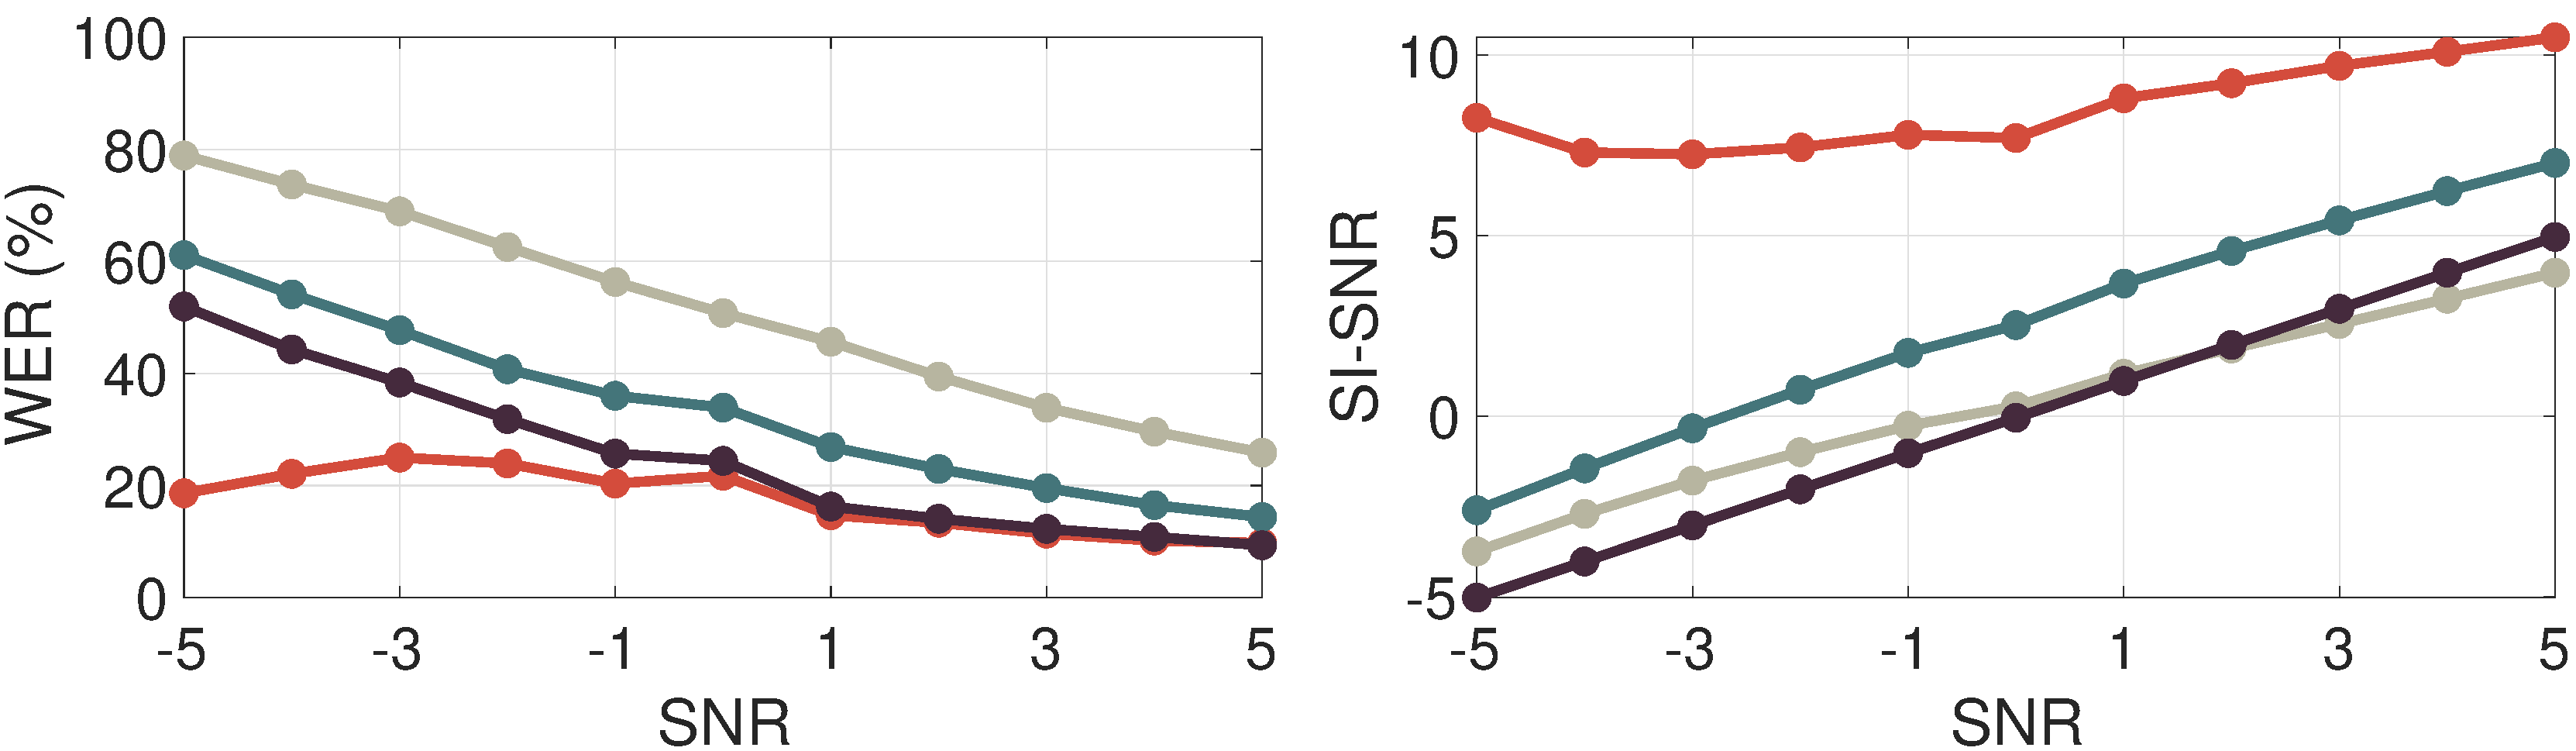
\includegraphics[width = \linewidth]{images/denoising_digital.pdf}
    \end{subfigure}
    
    \begin{subfigure}[t]{\linewidth}
        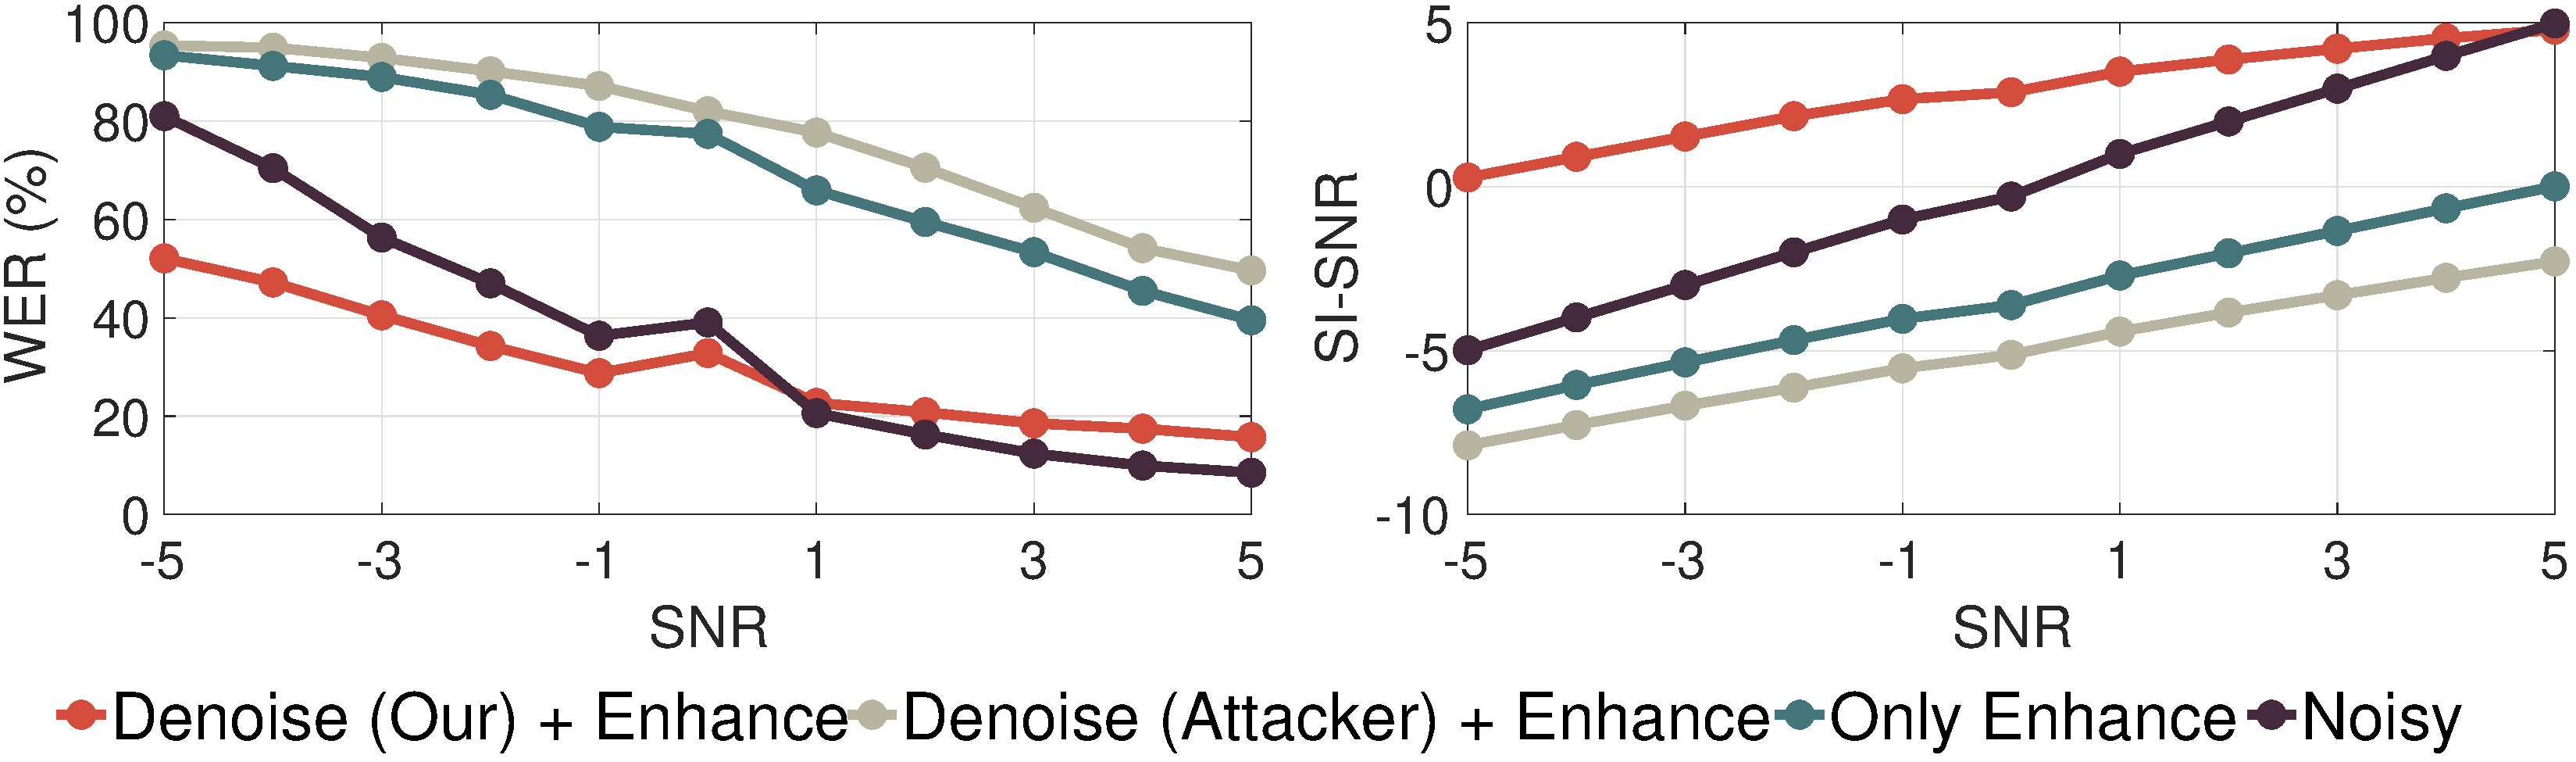
\includegraphics[width = \linewidth]{images/denoising_real_world.pdf}
    \end{subfigure}
    \caption{Result of content recovery. Top: digital scenario. Bottom: real-world scenario.}
    \label{fig:content_recovery}
    \vspace{-5mm}
\end{figure}

\subsection{Robustness Against Various Attackers}
\label{subsec:robustness}
Here we evaluate the robustness of our system against attackers with different capabilities. We consider two types of attacker: the \textbf{normal attacker} who has no knowledge of our jamming method and the \textbf{advanced attacker} who knows the details of our jamming method. We conduct experiments under different attack scenarios and the results show that our system can resist both types of attackers effectively.

\textbf{Normal Attacker with SOTA Speech Enhancement.} We first consider the attacker who has no knowledge of our system and could only use existing enhancement methods to improve the intelligibility of audio recordings. Here we consider a SOTA speech enhancement algorithm~\cite{hao2020fullsubnet} and enhance the speech signal obscured by different types of noise before recognition. We first employ WeNet for recognition and observe a notable improvement in accuracy for the WGN jamming case, surpassing $30\%$ in average, as shown in Figure~\ref{fig:digital_enhanced}. While for our noise, the accuracy decreases significantly after enhancement. We then further employ Tencent ASR and results show that the accuracy drops substantially after enhancement for both our noise and WGN. We speculate the decrease is caused by the conflict between Tencent ASR inherent speech enhancement and~\cite{hao2020fullsubnet}.

\begin{figure}[t]
    \centering
    \begin{minipage}[t]{0.49\linewidth}
        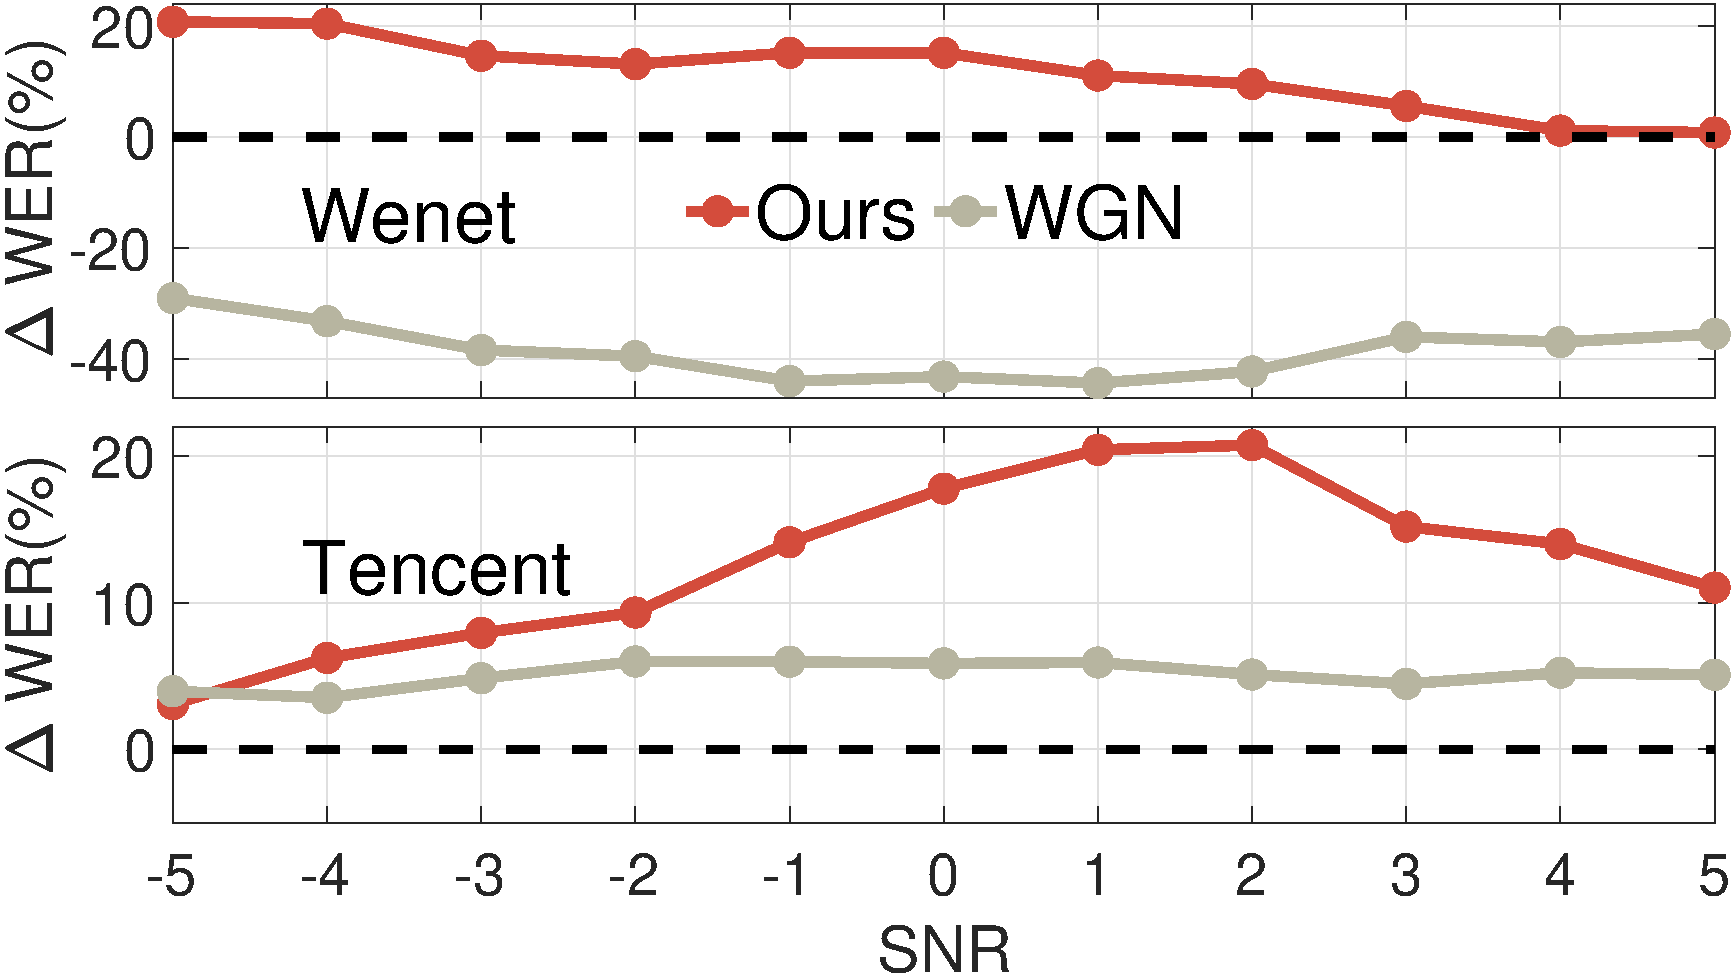
\includegraphics[width=\linewidth]{images/digital_enhanced.pdf}
        \caption{Recognition results after speech enhancement.}
        \label{fig:digital_enhanced}   
    \end{minipage}
    \begin{minipage}[t]{0.49\linewidth}
        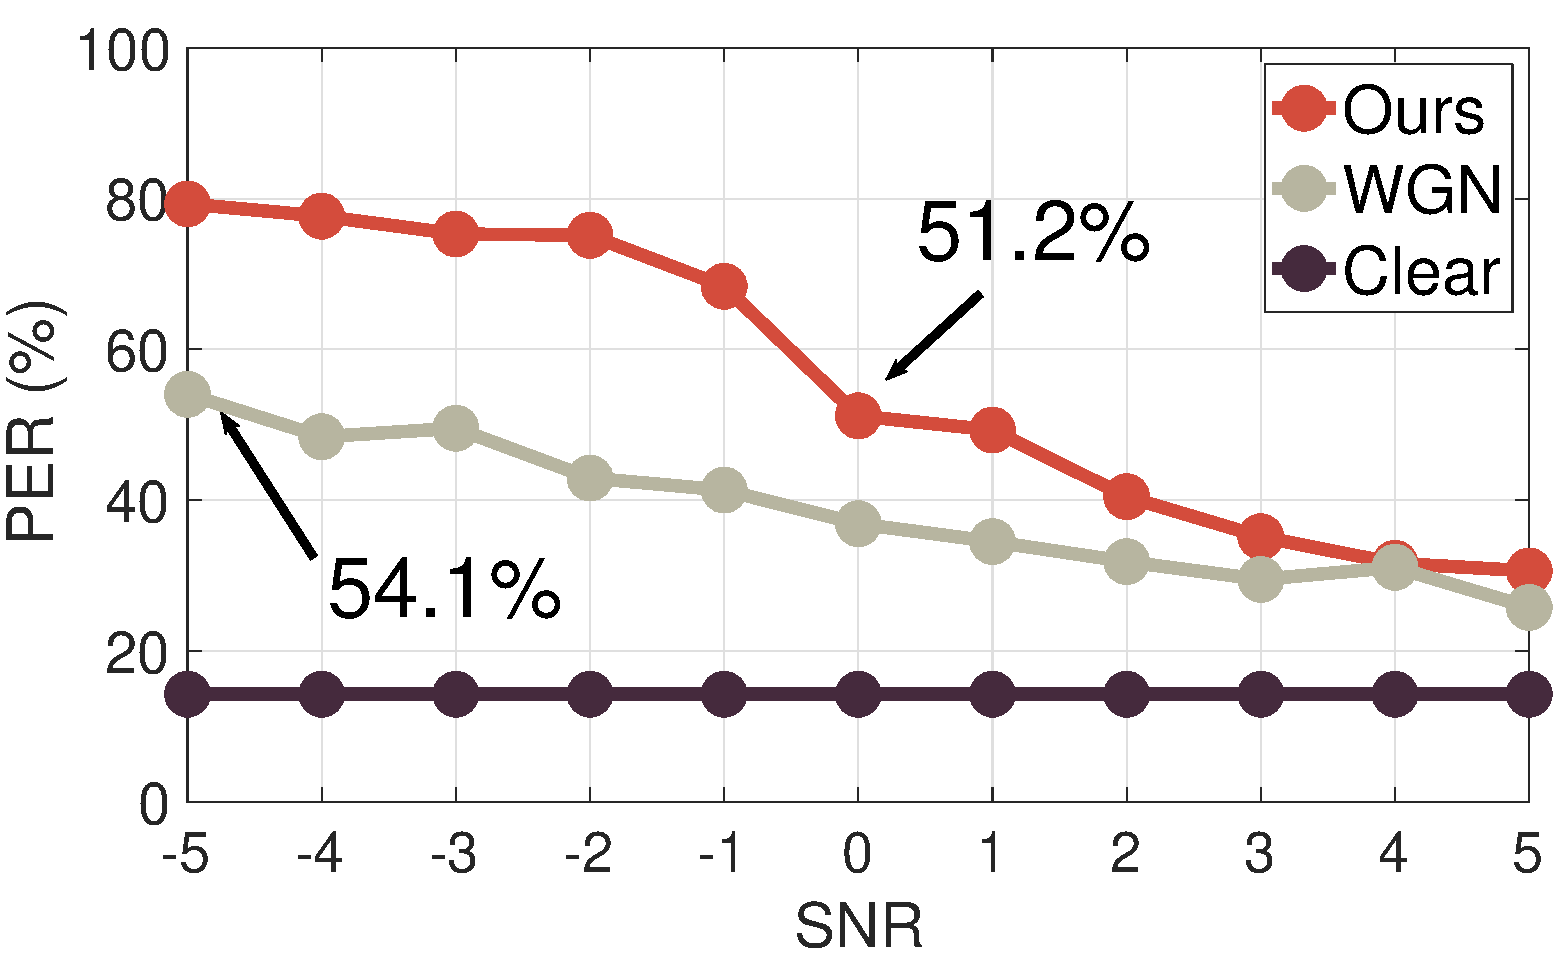
\includegraphics[width=\linewidth]{images/specific_deep_learning.pdf}
        \caption{PER of specialized ASR systems.}	
        \label{fig:train_targeted_ASR}
    \end{minipage}
    \vspace{-5mm}
\end{figure}

We further evaluate our noise robustness with the data collected in real-world scenario. The same enhancement method as before is used here and the result is shown in Tab~\ref{tab:real_world_enhanced}. Similar to the results in digital domain, the enhancement process reduces the recognition accuracy at each SNR.

\begin{table}[h]
    \caption{Robustness in real-world scenario against speech enhancement method}
    \centering
    \resizebox{\columnwidth}{!}{
        \begin{tabular}{cccccccc}
        \toprule
        \textbf{SNR}         & \textbf{\textless{}-4} & \textbf{{[}-4,-2{]}} &\textbf{ {[}-2, 0{]} }&\textbf{ {[}0,2{]}} &\textbf{{[}2,4{]}} & \textbf{\textgreater{}4 }\\ 
        \midrule
        \begin{tabular}[c]{@{}c@{}}Avg WER(\%)\\ (with Enhancement)\end{tabular} & 87.1          & 87.6        & 82.9        & 79.1      & 65.3      & 53.7\\ 
        \begin{tabular}[c]{@{}c@{}}Avg WER(\%)\\ (without Enhancement)\end{tabular} & 85.8          & 81.6        & 77.6        & 70.2      & 56.4      & 42.3\\ 
        \bottomrule
        \end{tabular}
    }
    \label{tab:real_world_enhanced}
\end{table}

\textbf{Advanced Attacker with Customized Speech Enhancement.} We then consider an advanced attacker that knows the detail of our jamming method. Instead of adopting existing enhancement methods, this attacker can train a model targeting on enhancing recordings jammed by our noise. Specifically, we consider the scenario described in Subsection~\ref{subsec:effectiveness_of_content_recovery}. The attacker creates a large speech dataset based on our jamming method and then trains the network as illustrated in Figure~\ref{fig:network_architecture} (without noise ref). Results in Figure~\ref{fig:content_recovery} (attacker part) shows that both the recognition accuracy and the audio quality (SI-SNR) decrease after speech enhancement, which means the advanced attacker can not recover the content from noisy recordings.

\textbf{Advanced Attacker with Specialized ASR.}
\label{subsec:robustness_adversarial_training}
We then consider an advanced attacker who targets on training a specialized ASR to recognize the noisy recording directly instead of enhancing it. Similar as before, We assume the attacker can create a large-scale dataset with our jamming method and train an ASR system from scratch. We choose TIMIT~\cite{timit} as the training data and take CRDNN~\cite{speechbrain} as the network architecture for its SOTA performance in speech recognition on TIMIT. The metric used here is PER (Phoneme Error Rate, similar to WER). We compare the recognition accuracy of specialized ASRs trained to recognize our noise and white noise respectively. Specifically, we train multiple ASRs and each one takes jammed speech signals with a specific SNR as the training data. As last, we have 22 ASRs considering the combinations of two types of noise and 11 SNRs.

The results are shown in Figure \ref{fig:train_targeted_ASR}. For white noise, the PER rises slowly with the decrease of SNR, which indicates the network's denoising ability for white noise. For our noise, the PER is slightly higher than white noise when $SNR\geq 0$, but increases rapidly when $SNR < 0$. These results mean that even when the attacker can train a specialized ASR, it is hard to recognize the audio jammed by our noise when $SNR \leq 1$, which is a reasonable value in real-world scenarios. We also find that when $SNR<0$, the training for the ASR targeting our noise can not converge properly for many reasons (e.g., exploding gradients), and requires careful parameter tuning.


\subsection{Comparisons with the Speech Noise}
\label{subsec:comparison_with_speech_noise}
In this part, we compare our noise with speech noises that contain 1, 2, and 3 speech series respectively. For a fair comparison, the speech series making up the noise is from the same people as the target. The results on the left of Figure~\ref{fig:test_sep} show that without considering noise reduction methods, our noise performs better when $SNR<-2$.

We then test the robustness of the noises against speech separation algorithms~\cite{sepformer} and trained three models targeting on noises containing 1, 2, and 3 series respectively. During the experiment, we find that although the separation process improves the intelligibility of audio for the human ear, the recognition accuracy of ASR is even worse than before. We think this is caused by the noise residue. So we further process the separated results with speech enhancement methods~\cite{fullsubnetPlus}. For our noise, we try to separate it with all three models separately then apply the enhancement. The result with the lowest WER is chosen for comparison. 

The result on the right of Figure~\ref{fig:test_sep} shows that when $SNR \ge 0$, the WERs of different tested noises are close; when $SNR<-1$, the WERs of speech noises with all SNRs are lower than 50\% and our noise performs much better. The result also reveals a phenomenon that higher noise energy for the speech noise does not always mean higher WER, which is different from our noise. Instead, the jamming performance of the speech noise will decrease when its noise energy is above certain threshold. The corresponding SNR thresholds are about 1, -3, and -4.8 for the noise containing 1, 2, and 3 speech series respectively. This phenomenon indicates that compared to our noise, the speech noise is less applicable in the real-world scenario as it is hard to control the noise energy to stay within a specific range.


\begin{figure}[t]
    \centering
    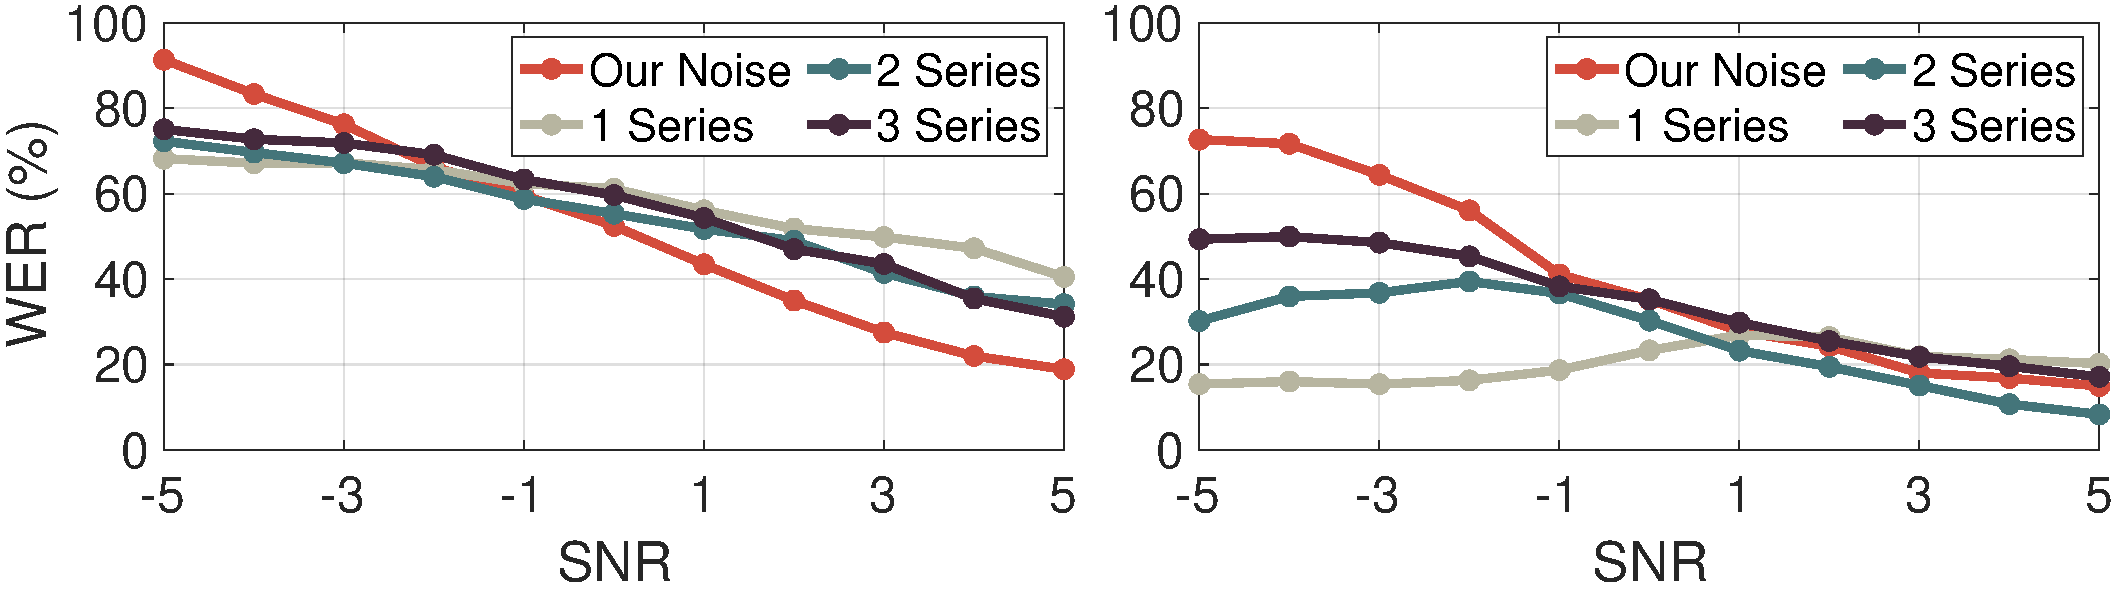
\includegraphics[width=\linewidth]{images/test_sep.pdf}
    \caption{Comparisons with speech-like noise. Left: WER before noise reduction. Right: WER after noise reduction.}
    \label{fig:test_sep}
    \vspace{-3mm}
\end{figure}

\subsection{Comparisons with Other Jamming Methods}
Here we compare our noise with the counterparts in two other related works, namely Backdoor~\cite{backdoor} and Patronus~\cite{patronus}, and a commercial off-the-shelf device~\cite{commercial_device}. The noise in~\cite{patronus} consists of dynamic frequencies and chirps. The range of frequency is $[50, 40k]$ Hz and the duration of signal in each frequency is 0.2s. The noise in~\cite{backdoor} is a band-limited (i.e., $[0, 12k]$) white noise modulated by a $40$ kHz carrier. As for the commercial device~\cite{commercial_device}, we do not have the knowledge of its internals, therefore we can only speculate that its noise is made of variable multi-frequency tones based on the spectrogram. We conduct this experiment in the real-world scenario. We play audios with a smartphone and play noises with our transmitter (except for~\cite{commercial_device}) with constant power in the meantime. Then we record the audio with one smartphone placed at different distances from the transmitter. The recordings are enhanced with different methods before being fed into an ASR for better recognition (the same process as~\ref{subsec:comparison_with_speech_noise} for our noise and FullSubNet+~\cite{fullsubnetPlus} for others). The results in Figure~\ref{fig:comparison_with_other_noise} show that our noise performs better than others significantly.

\subsection{Impact of Data Augmentation Process}
% As described in Section~\ref{sec:system_design}, the data augmentation module is designed for defending against the powerful attacker who can locate the recurrent patterns in the jammed recordings and so recover part of the semantic information in the audio. 
Here we evaluate the impact of the data augmentation process on the effectiveness of our noise. In the noise generation process, before concatenating a newly selected phoneme data in to the noise, for each augmentation method, the phoneme data would be augmented with a probability $p$.
% the phoneme data will have a probability $p$ to be augmented. 
Then we test the jamming effectiveness of the noise generated with different $p$. The results in Figure~\ref{fig:impact_of_augmentation} show that as $p$ increases, the jamming effectiveness of our noise gradually decreases. However, the impact is limited, with only a drop of 5\% in WER when $p$ increases form 0 to 0.5.

\begin{figure}[t]
    \centering
    \begin{minipage}[t]{0.49\linewidth}
        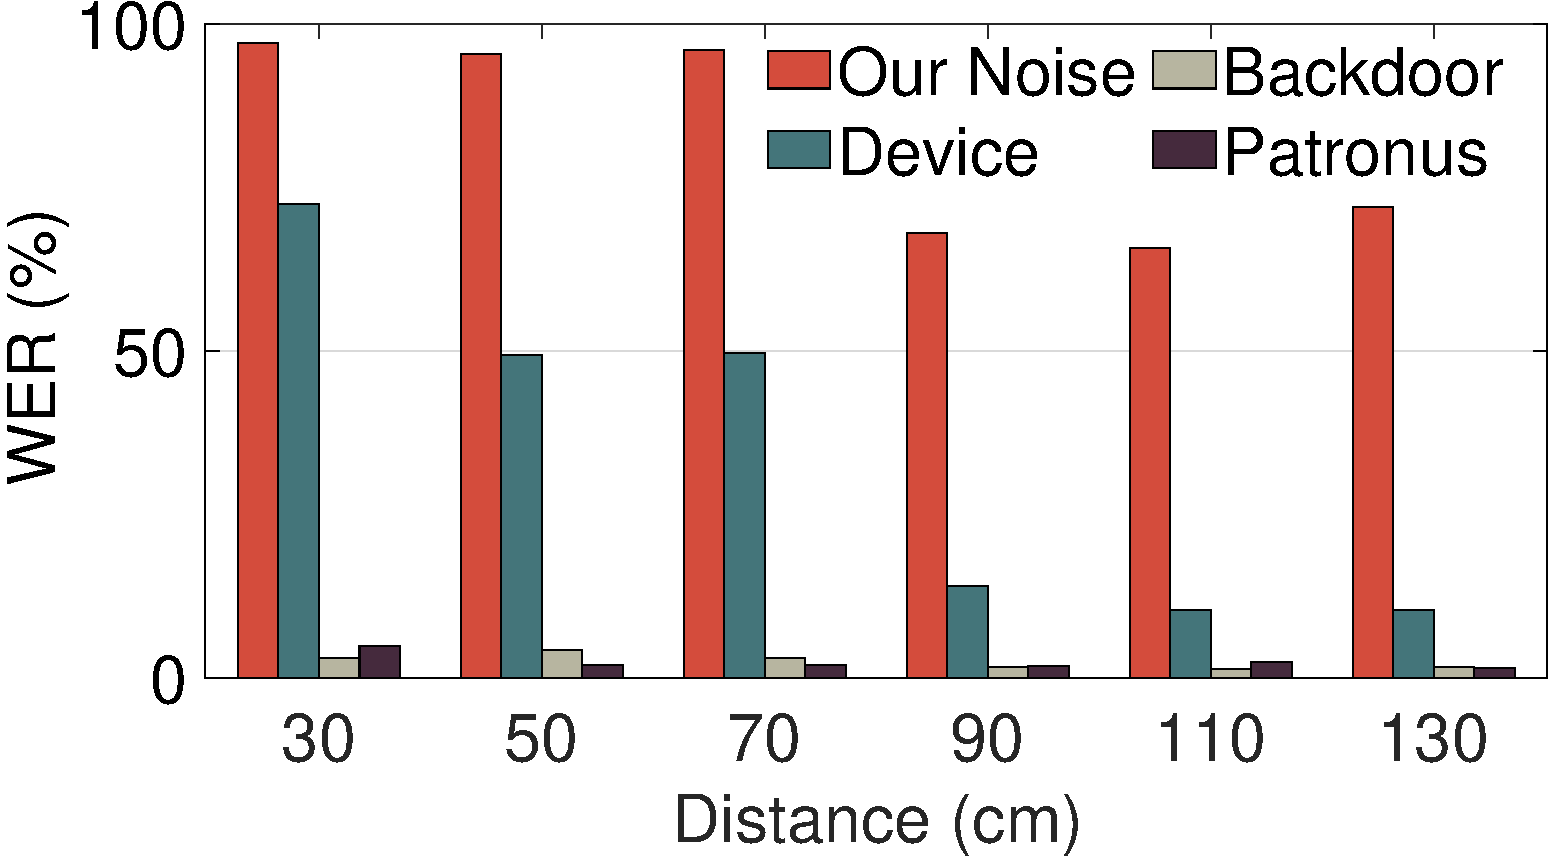
\includegraphics[width = \linewidth]{images/compare_sota.pdf}
        \caption{Comparisons with other existing methods}
        \label{fig:comparison_with_other_noise}
    \end{minipage}
   \begin{minipage}[t]{0.49\linewidth}
        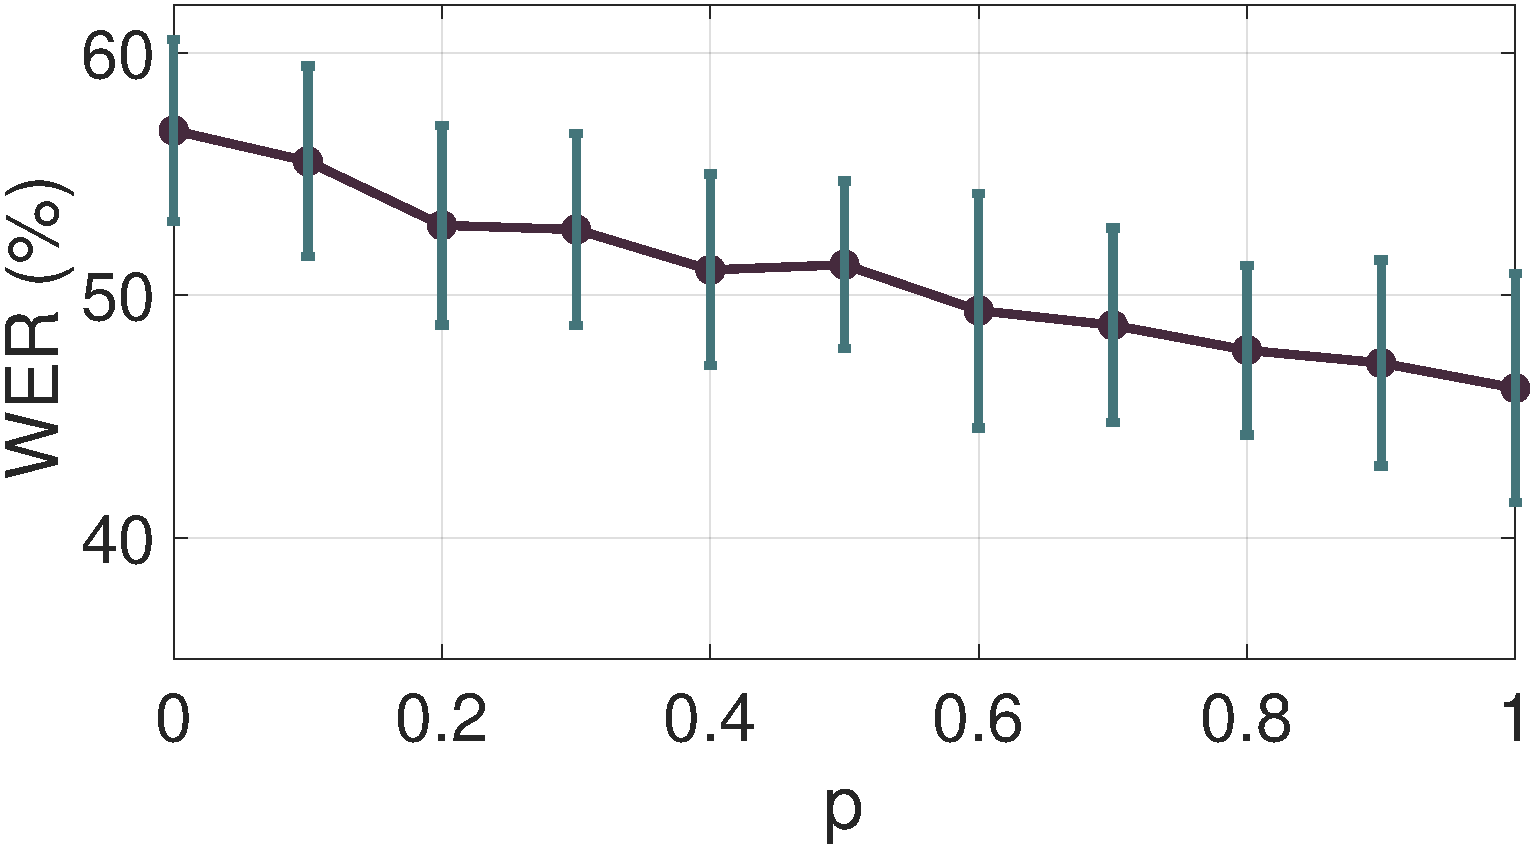
\includegraphics[width = \linewidth]{images/test_data_augmentation.pdf}
        \caption{Impact of data augmentation}
        \label{fig:impact_of_augmentation}
    \end{minipage}
    \vspace{-5mm}
\end{figure}

\subsection{Impact of Recording Devices}
\label{subsec:impact_of_recording_devices}
To test the generalizability of InfoMasker among different recording devices, we use different appliances to record demodulated signals and them calculate their energy. We test a variety of recording devices, including nine models of smartphones, an iPad, a smart watch, a smart home device and a laptop. Besides, we also test the nonlinearity of twelve smartphones of the same model (Samsung A51). The results in Figure \ref{fig:nonlinearity_in_diff_devices} shows the good generalizability of InfoMasker.

\begin{figure}[t]
    \centering
    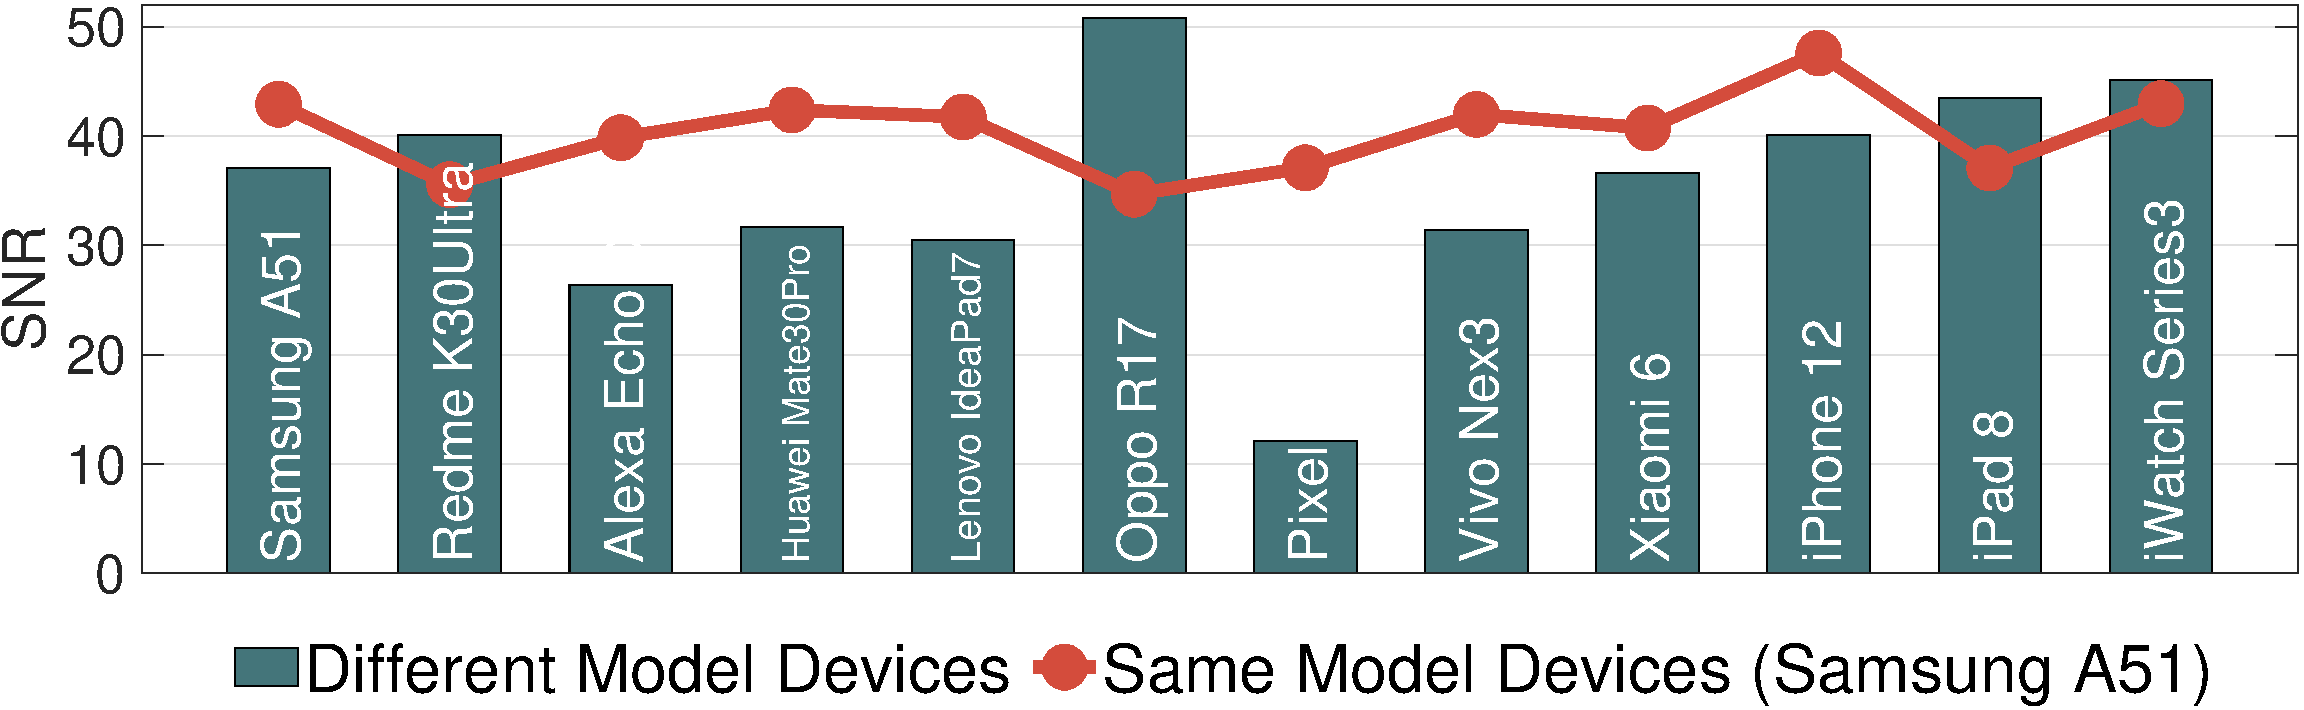
\includegraphics[width=\columnwidth]{images/non_linearity_diff_device.pdf}
    \caption{Nonlinearity in different recording devices}
    \label{fig:nonlinearity_in_diff_devices}
    \vspace{-3mm}
\end{figure}

\subsection{Case Study: A Common Office}
\label{subsec:case_study}
\textbf{Environment Setting.}
We further explore the possibility of deploying our system in a real-world environment. We deploy our system in a common office room, which is 6.2 meters long and 3.4 meters wide, as shown in Figure \ref{fig:environment}. We place a transmitter array in each of the four corners of the room. We first measure the ultrasound energy distribution in the room, and the result is shown in Figure \ref{fig:room_distribution}. 

Except for some areas within 10cm from the transmitter array, where the ultrasound energy reaches about 105 dB SPL, the energy in all other areas is lower than 95 dB SPL. This energy distribution meets the suggestion proposed by World Health Organization (WHO) that when humans are exposed to 40kHz ultrasound for more than 4 hours, the energy of the ultrasound should not exceed 110 dB SPL \cite{human_ultrasound_tolerance}.
\begin{figure}[t]
    \centering
    \begin{subfigure}[b]{0.39 \columnwidth}{
        \centering
        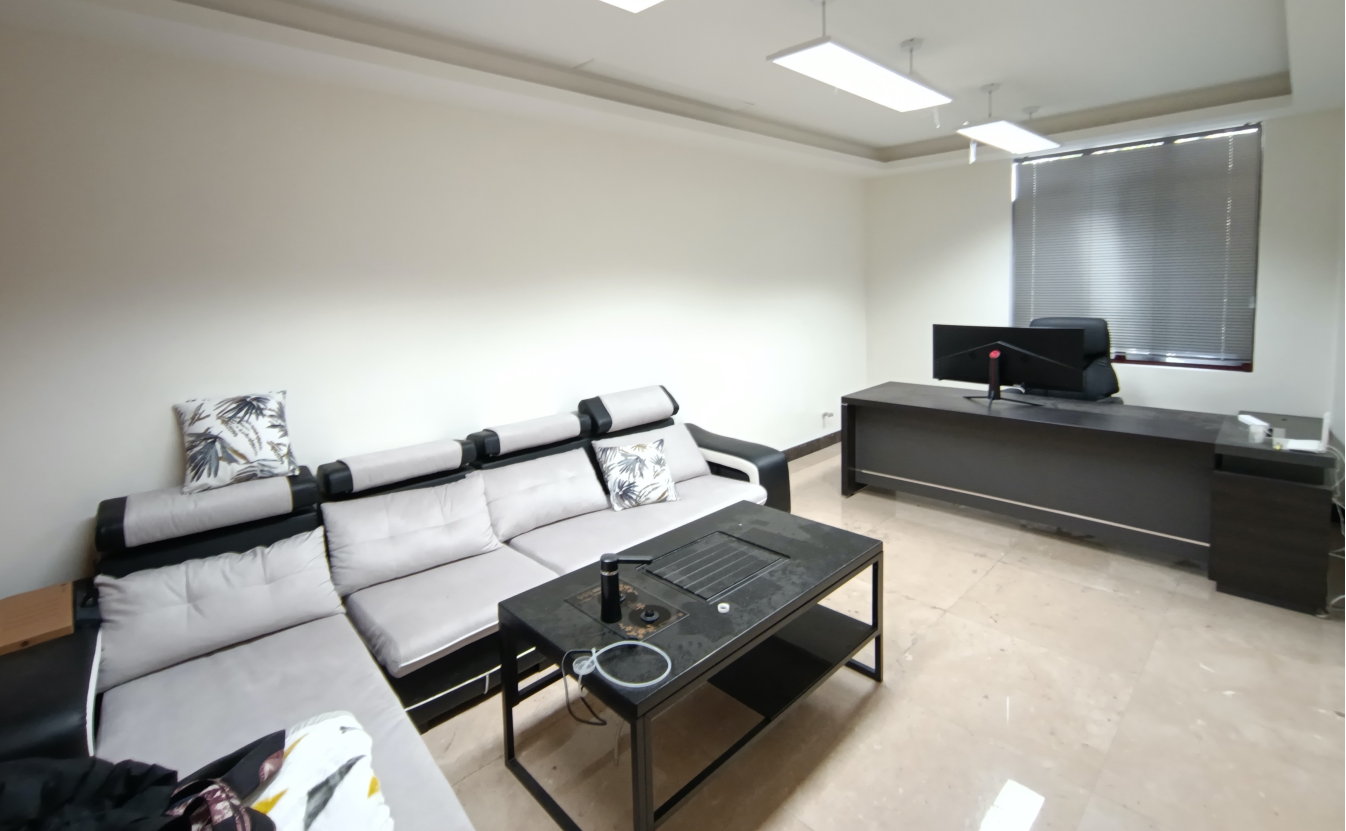
\includegraphics[width=\linewidth]{images/environment.pdf}
        \caption{The office.}
        \label{fig:environment}
    }
    \end{subfigure}
    \begin{subfigure}[b]{0.59 \columnwidth}{
        \centering
        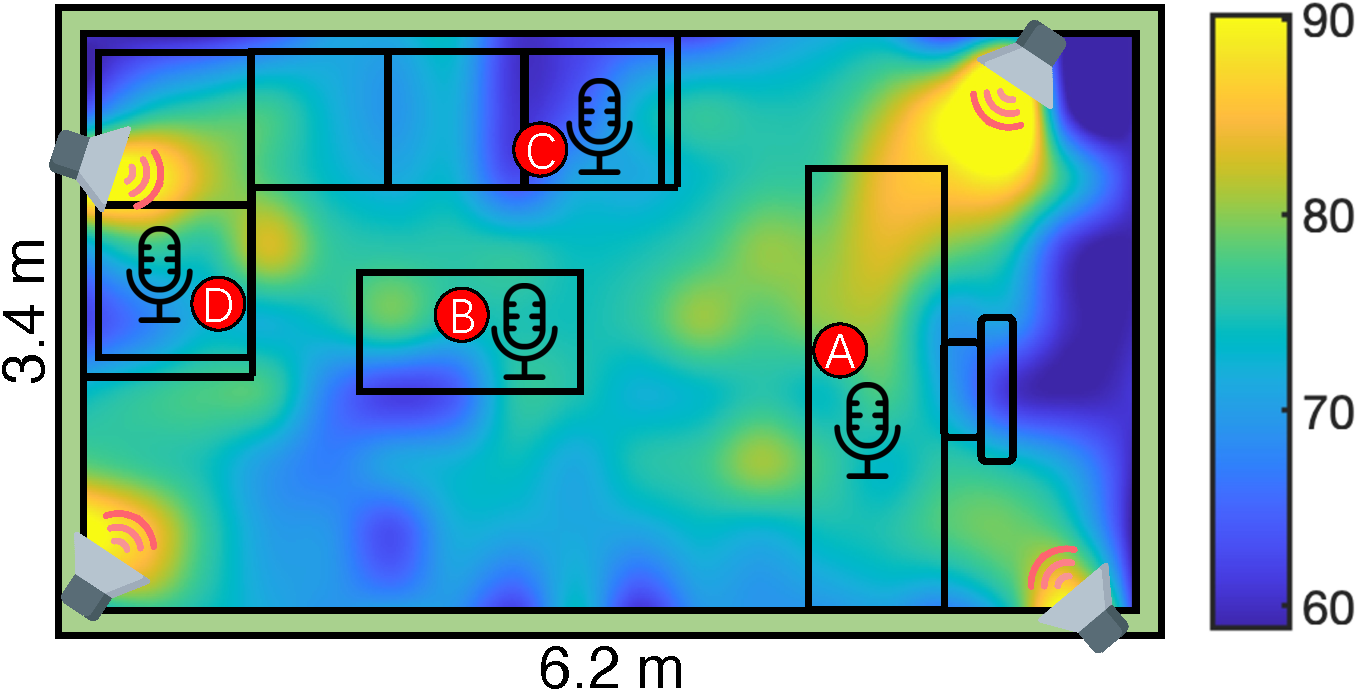
\includegraphics[width=0.8\columnwidth]{images/room_distribution.pdf}
        \caption{Energy Distribution.}
        \label{fig:room_distribution}
    }
    \end{subfigure}
    \caption{Experiment Settings.}
    \label{fig:equipment_environment}
    \vspace{-5mm}
\end{figure}

\textbf{Recognition Results.}
We place four devices in the positions highlighted in red in Figure \ref{fig:room_distribution}. The noise energy in Point A and B is relatively high and is relatively low in Point C and D. The devices placed include two smartphones (Samsung A51 and Huawei Mate30Pro), a laptop (Lenovo IdeaPad7), and an iPad (iPad8). For each device we record about 3 hours data and the result is shown in Figure~\ref{fig:case_study}(top). We use three commercial ASR systems to recognize each data and choose the lowest WER as the result. For the reason that the power amplifiers will generate audible noise when turned on, we also test the scenario where the power amplifiers are turned on but no noise is transmitted.

\begin{figure}[t]
    \centering
    \begin{minipage}[t]{0.8\linewidth}
        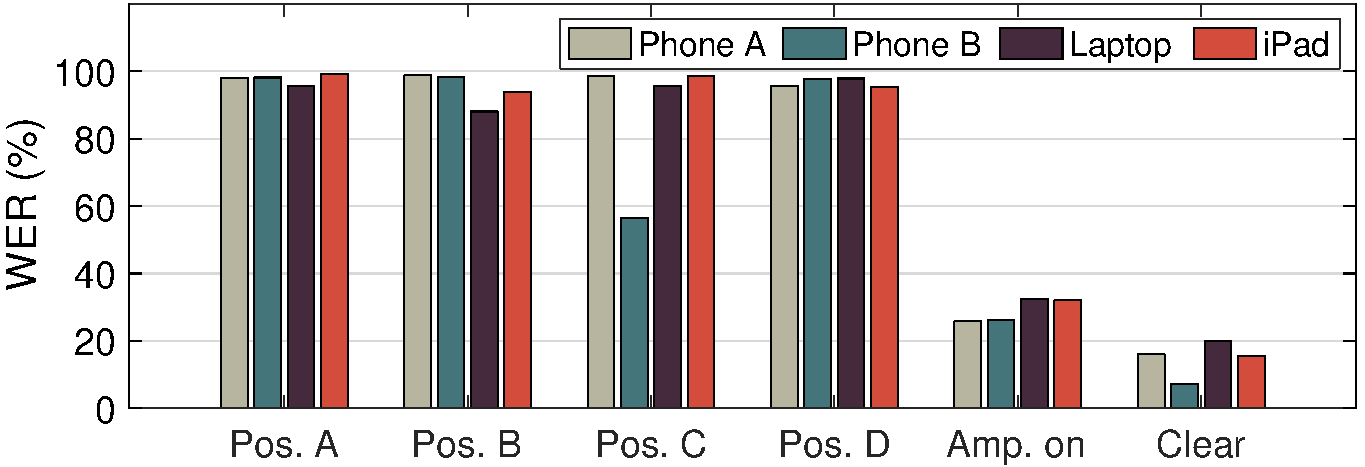
\includegraphics[width = \linewidth]{images/case_study_rec.pdf}
    \end{minipage}

   \begin{minipage}[t]{0.8\linewidth}
        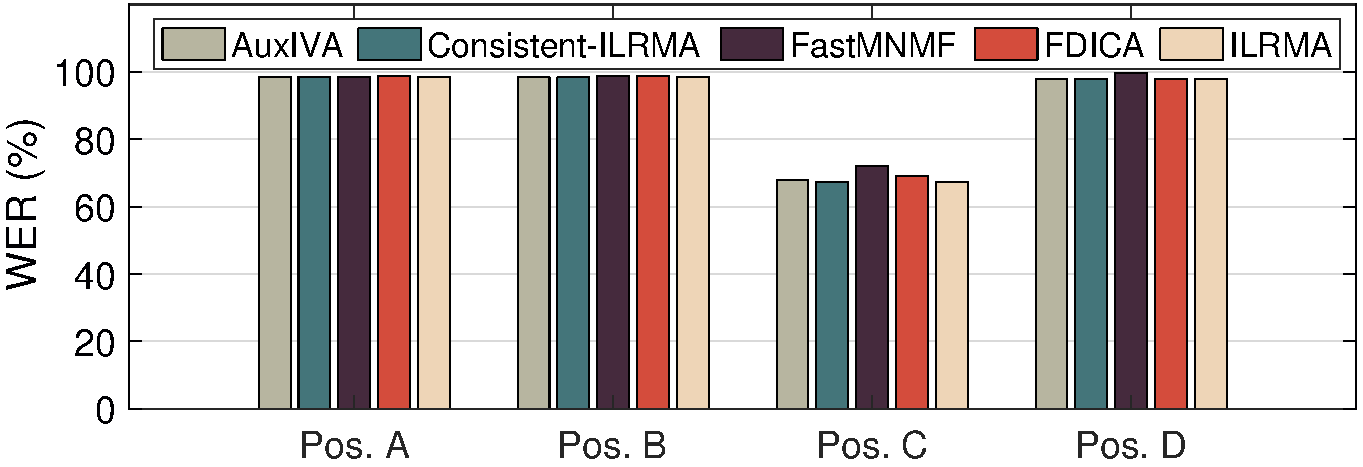
\includegraphics[width = \linewidth]{images/case_study_bss.pdf}
    \end{minipage}

    \caption{Top: Recognition results for the case study. Bottom: Recognition results after BSS (Phone B).}
    \label{fig:case_study}
    \vspace{-5mm}
\end{figure}

\textbf{Blind Signal Separation.}
Considering the recording device may have multiple microphones or there are multiple devices recording at the same time, the attacker could use BSS methods to denoise the recordings. In the case study, the recordings from the Huawei Mate30Pro have two channels, so we test the effectiveness of BSS on these recordings. We test five BSS algorithms: AuxIVA \cite{AuxIVA}, ConsistentILRMA \cite{consistentILRMA}, FastMNMF \cite{fastMNMF}, LaplaceFDICA \cite{fdica}, and t-ILRMA \cite{ilrma}. The results are shown in Table~\ref{fig:case_study}(bottom). It can be noticed that even at position C, where the noise energy is the lowest, BSS still cannot improve the recognition accuracy.